
%(BEGIN_QUESTION)
% Copyright 2011, Tony R. Kuphaldt, released under the Creative Commons Attribution License (v 1.0)
% This means you may do almost anything with this work of mine, so long as you give me proper credit

A byproduct of the {\it kraft process} used in the paper industry for turning wood chips into pulp is a liquid called {\it black liquor}.  This liquid contains many volatile sulfur compounds such as hydrogen sulfide (H$_{2}$S) and mercaptans, both of which are strongly scented, and if released to the atmosphere will constitute a hazardous (or at least strongly objectionable) emission.  Loss of volatile sulfur compounds also constitutes a loss of sulfur, which is a raw material in the kraft pulping process.

These sulfur compounds may be stabilized for less volatility and easier recovery by a process of oxidation: exposing the black liquor to pure oxygen gas.  To minimize consumption of oxygen, the gas flow is metered proportionately to liquor flow in a ratio control system:

$$\includegraphics[width=15.5cm]{i00435x01.eps}$$

One problem with this system, though, is that the purity of the oxygen gas varies over time.  Some days it is near 95\% pure, while other days it may sink down to 80\% purity.  The balance is made up of nitrogen gas, which does nothing to oxidize the liquor.  Operations personnel discovered this problem when they had an oxygen analyzer installed on the O$_{2}$ line coming in to the oxidation reactor.  Now they want a control system that takes this on-line measurement and automatically compensates the gas flow in to properly oxidize the liquor no matter what the oxygen concentration happens to be.

A useful problem-solving technique to apply here is a ``thought experiment'' where you imagine the oxygen purity changing between two easy-to-calculate values: suppose the purity begins at 100\%, then suddenly changes to 50\%.  How should an automatic compensating system respond to the O$_{2}$ purity {\it being cut exactly in half}, in order to maintain proper oxidation of the liquor?  Then, take that conclusion and implement it using one or more additional function blocks.

\vskip 20pt \vbox{\hrule \hbox{\strut \vrule{} {\bf Suggestions for Socratic discussion} \vrule} \hrule}

\begin{itemize}
\item{} Explain how the suggested thought experiment makes this a relatively easy problem to solve.
\item{} For those who have studied flow measurement, explain why each flow transmitter has {\it square root} characterization.
\end{itemize}

\underbar{file i00435}
%(END_QUESTION)





%(BEGIN_ANSWER)

The optimal solution uses a {\it divider} function block rather than a summer, so that the feedforward oxygen analyzer's signal will have the proper multiplicative effect on oxygen flow to the reactor if the oxygen purity becomes weakened:

$$\includegraphics[width=15.5cm]{i00435x02.eps}$$

If oxygen concentration were to fall from 100\% to 50\% (for example), we would need {\it twice} the flow rate of oxygen to the reactor than previously, not just an additional sum of oxygen flow.

%(END_ANSWER)





%(BEGIN_NOTES)


%INDEX% Control, strategies: feedforward
%INDEX% Control, strategies: ratio
%INDEX% Process: black liquor oxidation (Kraft pulping)

%(END_NOTES)


